\chapter{Introduction}

Since the dawn of democracy, elections have been accused for the lack of transparency and security. As societies all over the world are rapidly adopting technology across all aspects of society, a digitalized democratic system of voting might just be the next evolutionary step towards a transparent and trusted electoral system.

In this first chapter, we introduce our work on proposing a decentralized voting system.

\section{Background}

As the hype surrounding bitcoin\cite{satoshinakamotoBitcoinPeertoPeerElectronic} is slowly waning, the industry is becoming more and more interested in its underlying technology: the Blockchain. Now, proponents claim Blockchain technology to be one of the most important new technologies of our time, about to take society by storm, and bitcoin served as the first, most thorough and complete proof of concept. In fact, Marc Andreessen, founder of VC firm Andreessen Horowitz and one of the most influential members of Silicon Valley, claimed in a New York Times article that the invention of the Blockchain is as important and influential as the creation of the Internet itself\cite{andreessenWhyBitcoinMatters1390323270}.\smallskip

Along with assets registry, secure sharing of medical data and supply chain and logistics monitoring, electronic voting is one of the most prominent potential applications for the surging Blockchain technology.

\section{Key Concepts}

These are the most critical concepts that our work deals with.

\subsection{Voting}

According to Oxford English dictionary, voting (also known as election) is \textit{"a formal indication of a choice between two or more candidates or courses of action, expressed typically through a ballot or a show of hands"}, and the very first forms of voting date back to approximately 508 B.C in ancient Greece where the earliest form of democracy was implemented\cite{mikehoganHistoryElectionsOnline}. Greeks had a "negative" election -- that is, each year voters, who were the male landowners, were asked to vote for the political leader or "candidates" they most wanted to be exiled for the next ten years.

The early ballot system was voters wrote their choice on broken pieces of pots, ostraka in Greek, and from this name comes our present word to ostracize. If any "candidate" received more than 6,000 votes then the one with the largest number was exiled. If no politician received 6,000 votes then they all remained. Since voters were only male landowners, the number of voters was small. If there was a fairly even spread of votes, no one would be exiled, so usually, only very unpopular political leaders were ostracized or exiled.\cite{mikehoganHistoryElectionsOnline}

The election is the backbone of modern democratic societies, it often takes place at a polling station; it is voluntary in some countries, compulsory in others, such as Australia.

\subsection{Electronic voting}

Electronic voting (e-voting) is a security-critical application of electronic democracy (e-democracy). E-voting has become an applicable alternative for many non-governmental elections recently. There are a number of e-voting experiments currently being employed by various countries in political area as well. However many discussions, controversies and irregularities have been raised about them. The e-voting experience in Ohio in 2004 is one of the well-known examples which caused many discussions about vote miscount and modification. Therefore, it is not easy to say that an accurate and faultless e-voting is likely to become viable soon for governmental elections\cite{orhancetinkayaVerificationValidationIssues}.

E-voting is an inter-disciplinary subject and should be studied together with the experts of different domains, such as software engineering, cryptography, politics, law, economics and social sciences. Although many people have worked on this subject, mostly e-voting is known as a challenging topic in cryptography. The challenge arises primarily from the need to achieve voter anonymity, in other words to remove voter’s identity from his cast ballot in order to ensure voter privacy whereas ensuring the e-voting has been done correctly without any violation and ensuring only eligible voters’ votes have been counted. Thus, e-voting has been intensively studied in the last decades\cite{orhancetinkayaVerificationValidationIssues}.

\subsection{Blockchain technology}

A Blockchain is essentially a distributed database of records, or public ledger of all transactions or digital events that have been executed and shared among participating parties. Each transaction in the public ledger is verified by consensus of a majority of the participants in the system. Once entered, information can never be erased. The Blockchain contains a certain and verifiable record of every single transaction ever made\cite{michaelcrosbyBlockchainTechnologyBitcoin2016}.

\begin{figure}[h]
	\centering
		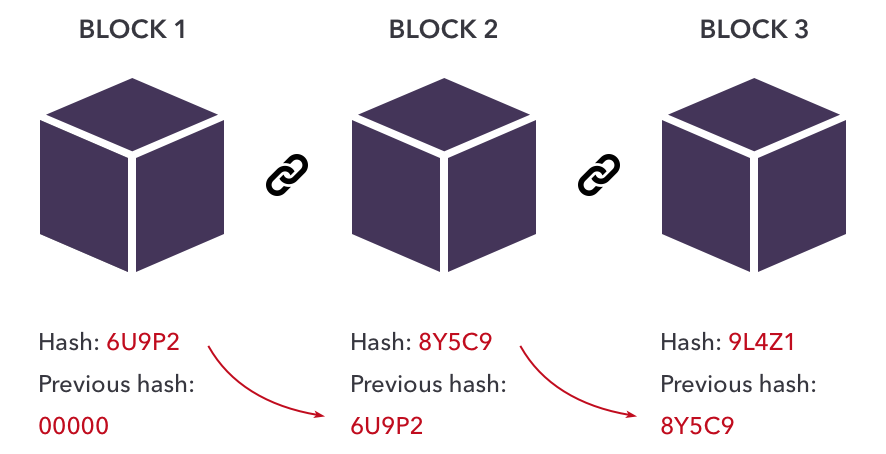
\includegraphics[width=10cm]{images/chapter1/blockchain.png}
		\caption{{\footnotesize Abstract Blockchain blocks visualization}}
\end{figure}

A Blockchain network can track orders, payments, accounts, production and much more. And because members of the network share a single view of the truth, you can see all details of a transaction end to end, giving you greater confidence, as well as new efficiencies and opportunities.\newpage

\section{Problem \& motivation}

Elections are expensive, complicated to set up and even on extreme cases fraudulent. This democratic system is almost 3000 years old and it has not evolved since ancient Greece. It entails an obligation for the voters to rely on third party officials and groups to safely collect votes and publish results, In the case of the modern democratic nation of France for example, there are only 3000 magistrates delegated to supervise and monitor more than 35 000 communes\cite{republiquefrancaiseArticleLO274Code2021}, a feat that is inconceivable for them to physically achieve, so setting the human malice apart still leaves room for human error, both leading to the voters carrying justifiable suspicions to any result the ballot may yield. Classic elections also carry hefty financial burdens, the 43rd general election (December 31st, 2020) of Canada had a total estimated cost of \$502.4 million\cite{electionscanadaEstimatedCost43rd2021}, the equivalent of the cost of building 5 new hospitals, including administrative areas, operating and emergency rooms, and space for 120 beds\cite{fixrcompanyCostBuildHospital2020}.

\begin{wrapfigure}[13]{r}{5cm}
	\vspace{-10pt}
	
\includegraphics[width=5cm]{images/chapter1/votomatic.jpg}
	\vspace{-10pt}
	\caption{{\footnotesize The Votomatic vote recorder, a punch card voting machine originally developed in the mid 1960s}}
	\label{votomatic}
\end{wrapfigure}

Then comes technology, the premise held while entering various fields is that it will increase efficiency, cut costs and leave all parties involved satisfied, with an abundance of examples of when technology did also keep that premise, voting seems to be a logical place to land in next. Electronic voting systems and semi-electronic ones existed for quite some time, from punched card systems {\small (see figure \ref{votomatic})} to modern-day digital voting machines. However, they only served to optimize the physical act of punching a card or putting a piece of enveloped paper in a box, although that did cut some costs, may be made the experience of voting more pleasant, but it introduced more security concerns and most importantly it did not solve the essential problem of eliminating third parties, because people still had to trust the hardware and software engineers that programmed the machines to cast the votes, and the servers to not allow for any tampering with the data.\newpage


\section{Purpose \& delimitations}
The goal of this research is to investigate the possibility of using the new surging Blockchain technology as the underlying technology powering an electronic voting system, offering the ability to store the results in a decentralized ledger that should grant the solution attributes like immutability and transparency. We intend to achieve our goal by designing a decentralized e-voting system as a \gls{proof-of-concept}, capable of launching an election, casting votes, and displaying results, all while ensuring transparency, anonymity, security and above all correctness of the results.
It is of major importance to define the scope of this research document and its underlying implementation.

First, the implementation of the proof of concept is not by any means complete and thorough but instead functionality was compromised in favor of delivering an actual election on the Blockchain.

Second, regarding Blockchain technology, this document will not dive deep into the inner workings of the technology, topics like hash functions, cryptography and proof of work mechanism will not be presented in a manner that debates their efficiency since we judge the scientific literature on these subjects to be of abundance, the focus will instead fall on how the application of this technology on voting would look like. Also as Asaf Ashkenazi said \textit{"Every device and system is hackable—it’s just a matter of time and hacker motivation."}\cite{leonhermonHowHackedLight2019} so our focus will not fall on defending the robustness of our implementation or any future implementation but rather it will fall on highlighting the promise that this technology presents in terms of robustness.
Lastly, code snippets that are unique to this project are included.

\begin{figure}[h]
	\centering
		
\includegraphics[width=4cm]{images/chapter1/verum.png}
		\caption{{\footnotesize Proof-of-concept "Verum" Logo}}
\end{figure}

\section{Document structure}
This document is presented in 5 chapters, starting with the chapter 1: Introduction, in which we present a bit of background of the topic and then delve into formally defining the problem we intend to tackle, followed by a brief description of what lies within and beyond the scope of this work.

In Chapter 2: Technical background, we present sufficient technical background about the two major aspects of our project, being the Ethereum Blockchain and Web applications. The next chapter, Chapter 3: Contribution \& system design. Next comes chapter 4: Implementation, a chaper about the implementation of our proof-of-concept, in which tools are introduced and results are displayed using diagrams, screenshots, and language.

Finally, in chapter 5: Conculusion and prespectives, the results and insights gained through the journey of making our proof-of-concept are discussed, few conclusions drawn and perspectives on what could be enhanced moving forward with this project.